\section{AOSP 概述}\label{aosp-introduction}

Android 由 “开放手机联盟” (Open Handset Alliance) 的开发者联盟开发,Google 对其提供商业赞助。为了开发更高效、更智能的移动端智能设备,Google 参考了若干开源移动端操作系统,开发了一套基于 Linux 内核改良版本开发的开源代码软件栈,这便是 Android\cite{PLATFORMARCHITECTURE}。Android 本身由两部分组成,一部分是大多数 Android 设备都预装的额外专有软件,其中包括 Google Chrome、数字发行平台 Google Play 和相关的 Google Play 服务开发平台,这些核心应用统称为 Google 移动服务 (GMS)。而另一部分则是遵守 Apache License 的免费开源软件,这一部分软件项目被统称为 AOSP,意为 “Android 开源项目”。

正由于 Android 是首个以打造完全开放和完整的移动端软件为目的的软件项目,Android 现在是全世界占有率最大的优秀移动操作系统。Android 项目完整覆盖了移动端从高端用户到低端用户的所有消费需求。对于有特殊需求的用户,Android 提供了对所有用户公开的文档、可由用户自定义的 Android 开源部分以及将用户修改移植到几乎所有设备的构建系统。

\subsection{Android 软件栈架构简述}

Android 是一套基于 Linux 内核改良版本开发的开源代码软件栈。Google 为适配各种移动端设备型号,将 Android 整体架构划分为五层——Linux 内核层、硬件抽象层、Android Runtime 与 C/C++ Lib、Java API 框架以及系统应用层。Android 软件栈架构图可见图 \ref{fig:android-stack}。

\begin{itemize}
    \item Android 软件栈的最底层是 Linux 内核部分,其利用 Linux 内核中的进程与线程管理、内存管理、设备管理、文件管理等功能,为上层的 Android 程序开发提供有效的平台基础。由于 Android 软件堆栈中的 Linux 内核部分可以利用 Linux 内核执行底层功能,因此,Android 有能力进一步为更高层的应用提供对基础功能的再抽象能力。
    \item Android 软件栈的第二层是硬件抽象层 (Hardware Abstraction Layer) 。硬件抽象层负责再包装 Linux 内核层提供的硬件能力。HAL 包含多个库模块,其中每个模块都为特定类型的硬件组件实现一个界面,例如相机和蓝牙模块。当框架 API 要求访问设备硬件时,Android 系统将为该硬件组件加载库模块。
    \item Android 软件栈的第三层是 Android Runtime 和 C/C++ Lib。对于运行 Android Lolipop(API 级别 21)或更高版本的设备,每个应用都在其自己的进程中运行,并且有其自己的 Android Runtime 实例。ART 编写为通过执行 DEX 文件在低内存设备上运行多个虚拟机,DEX 文件是一种专为 Android 设计的字节码格式,经过优化,使用的内存很少。编译工具链将 Java 源代码编译为 DEX 字节码,使其可在 Android 平台上运行。
    \item Android 软件栈的第四层是 Java API Framework。该层建立在底层 Android Runtime 和 C/C++ Lib 之上,为 Android 应用开发者提供应用开发所需要的工具与框架。Java API Framework 作为开发者可以直接且完全访问的 Android 系统应用使用的框架 API,封装了整个 Android 操作系统的所有功能。
    \item Android 软件栈的第五层是系统应用层。该层与用户直接交互,用于装载 Android 系统内置以及用户所开发的应用软件。
\end{itemize}

\begin{figure}[htb]
    \centering
    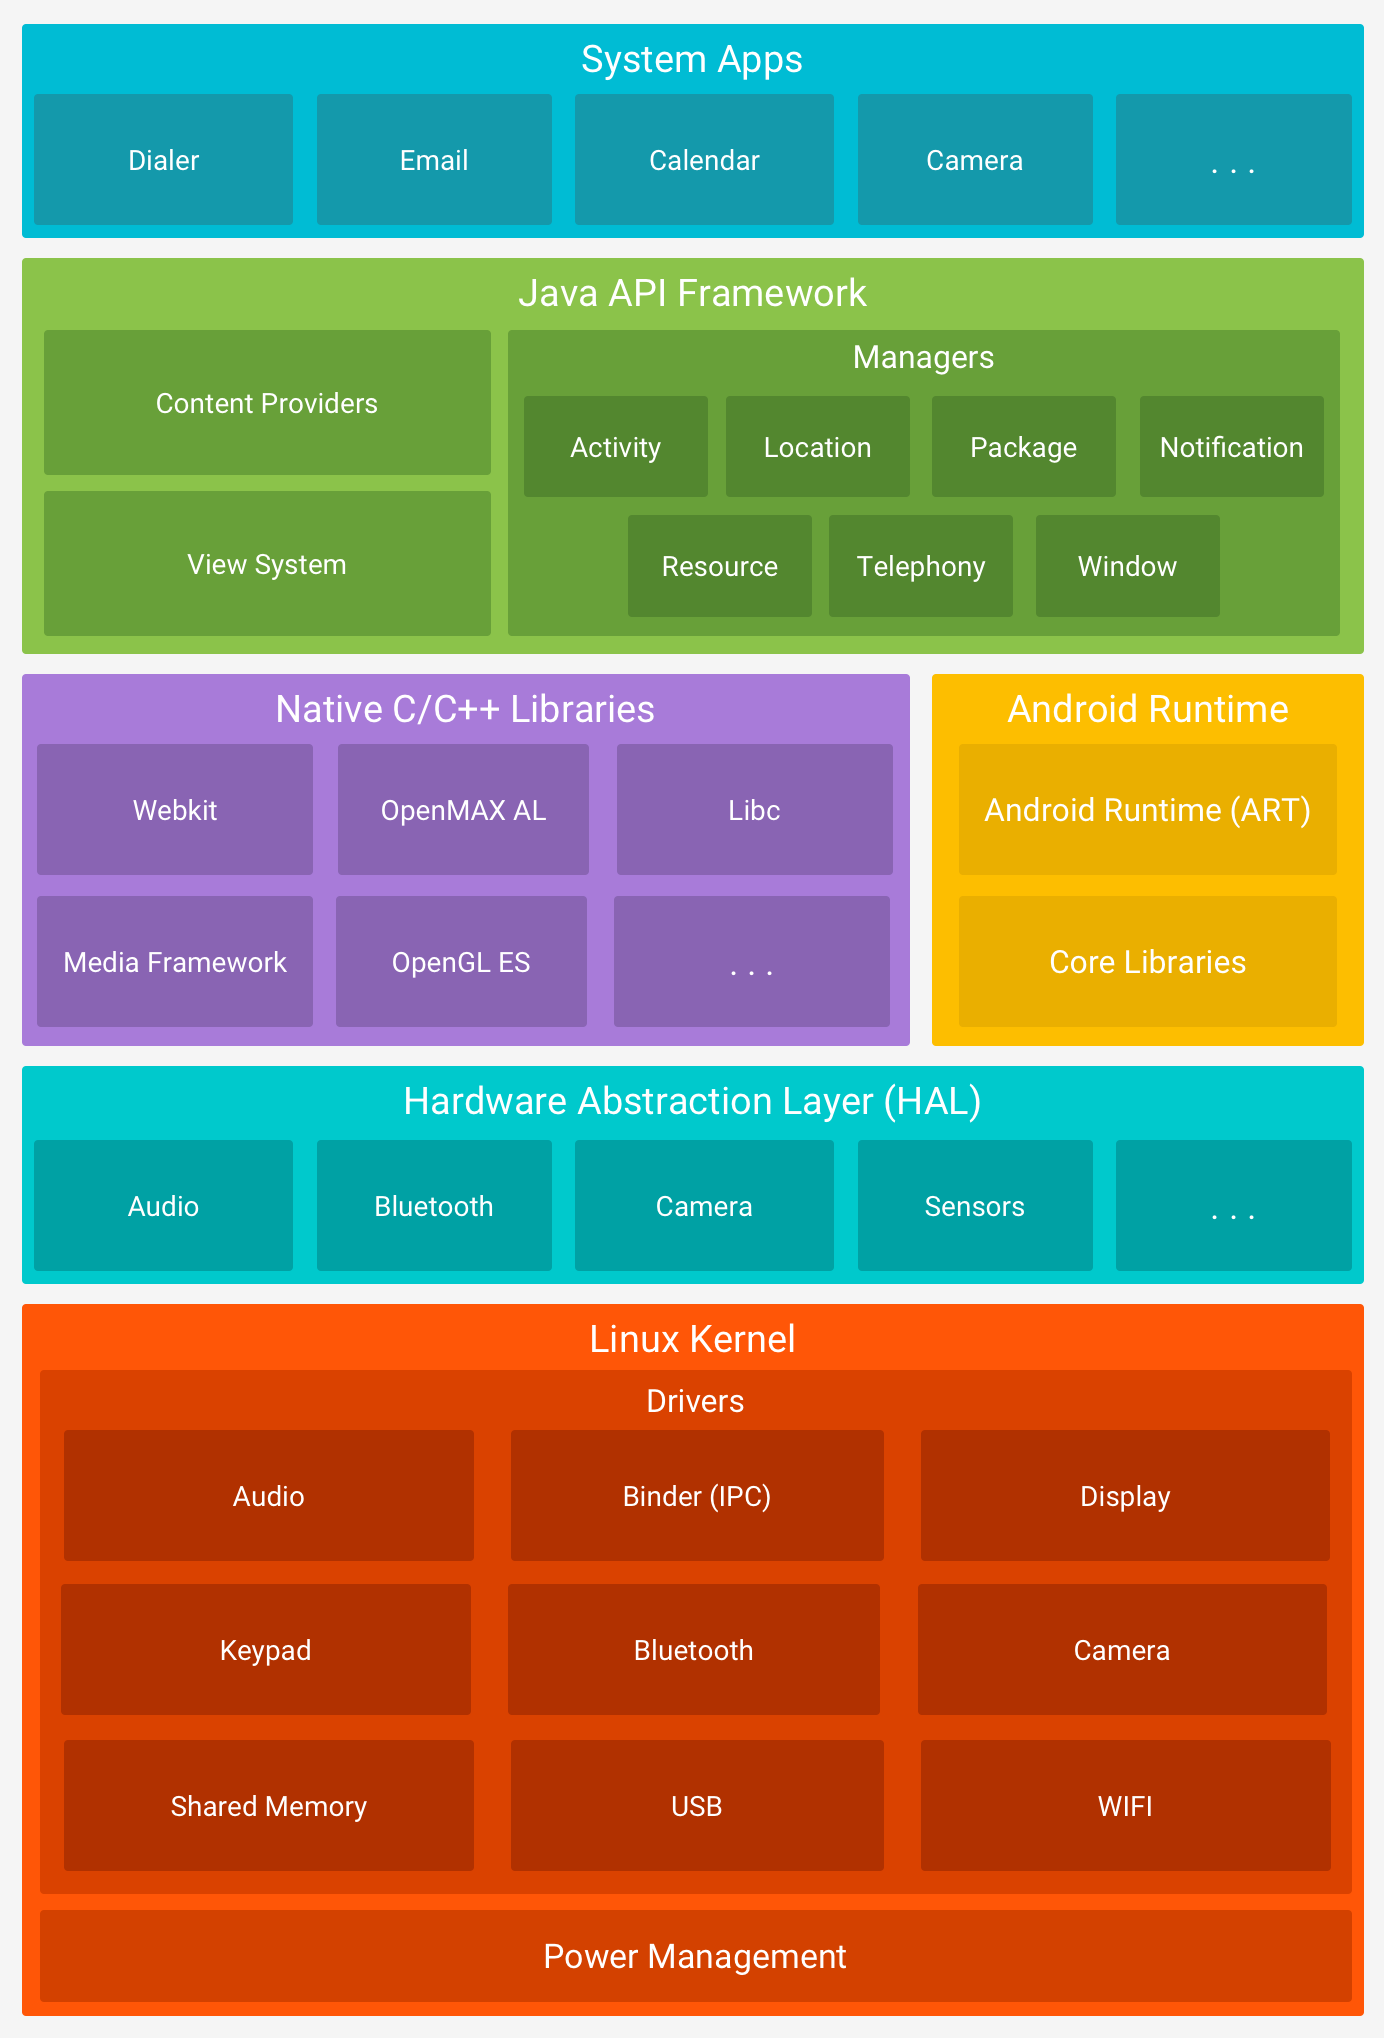
\includegraphics[width=.7\textwidth]{figures/android-stack_2x.png}
    \caption{Android 软件栈示意图}
    \label{fig:android-stack}
\end{figure}

\subsection{AOSP 构建系统历史与现状}

对 AOSP 展开分析的最重要一步是了解 AOSP 的构建过程,而 AOSP 构建系统是解释 AOSP 构建过程的核心关键。本节从 AOSP 构建系统从 GNU Make 到 soong 的演化历史出发,比较了二者在实际应用上的表现并介绍了 soong 中的重要组件与工作方式。

\subsubsection{Android Marshmallow 前:GNU Make}

截至 2015 年上半年,AOSP 所使用的构建系统仍旧依托于 GNU Make——各个模块通过编写各自的 Android.mk 文件,完成对 Android.mk 当前目录下所有源文件的编译以及最终产物的生成。在这一阶段,AOSP 为 GNU Make 提供了统一的编译入口,使用 Makefile 语言的指令将众多仓库下的模块一同构建。由于 GNU Make 的本质是执行给定指令,因此对于使用多种通用编程语言的 AOSP,GNU Make 是一个优秀的顶层构建系统。

然而,随着 AOSP 软件规模的不断增长,GNU Make 逐渐暴露出它的不足之处:

\begin{itemize}
    \item GNU Make 下的 Makefile 文件存在一定的逻辑语句,语法仍较为复杂。Makefile 语法较为灵活,存在诸如分支逻辑、循环逻辑等结构,这为项目开发人员以及软件分析人员带来的较大的困难。
    \item GNU Make 下的 Makefile 需要在每个模块构建之初消除先前模块构建过程中定义的环境变量所带来的影响,进而产生了大量必要且重复的 Makefile 代码。
    \item GNU Make 下的 Makefile 在 AOSP 庞大的系统下,很难在尽量降低对其他模块构建产生影响的同时,对特定模块进行定制化构建工作。
    \item GNU Make 在实际应用过程中,暴露出构建缓慢、难以统一管理等问题。
\end{itemize}

\subsubsection{Android Nought 后:soong / Ninja}

出于对以上问题的考虑,Google 决定将 AOSP Marshmallow 作为最后一个使用 GNU Make 为主要构建系统的大版本,并从 2015 年 1 月起开发适用于 AOSP 的新顶层构建系统——soong。与此同时,Google 采用 Ninja 这一已在 chromium 项目中得到认可的底层构建系统作为代替 GNU Make 构建图生成、构建时资源调度以及提供指令执行环境的工具。

自 Android Nought 开始,AOSP 的构建系统在逐渐从 GNU Make 向 soong / Ninja 过渡。截至目前,AOSP 仍旧存在使用 GNU Make 时期的 Android.mk 文件作为模块构建方式声明的 manifest 文件。

\subsection{soong 构建系统概述}

作为 AOSP 的顶层构建系统,soong 需要负责处理 AOSP 内部的复杂性。为了摒除 AOSP 内多语言项目间构建差异与各模块内与模块间引用带来的影响,soong 需要多个组件来完成整体构建过程。

\subsubsection{Blueprint}

在计划逐步抛弃 GNU Make 后,soong 同样需要一种用于描述 AOSP 中各模块内部与模块间的引用关系的文件协议。通过借鉴 Google 公司开发的另一个构建系统 “Bazel.build” 使用的 manifest 语法,soong 对其进行改造后设计形成了以 “bp” 为文件后缀名的 “Blueprint / Android.bp” 文件,用以替换原本各模块中的 Android.mk 文件。

目前,绝大多数模块使用 Android.bp 文件作为模块构建过程的声明文件(如 frameworks/base)。对 bp 文件格式的解析需要有一个独立的 Blueprint 模块完成,在当前版本的 soong 中,Blueprint 模块完成了对 bp 文件内容语法语义的解析。

相比于在较大程度上依赖于 AOSP 目录结构的 soong 构建系统而言,Blueprint 模块是一个十分独立的部件。这是由于 Blueprint 模块在设计之初,Google 公司希望设计一套能够独立于 AOSP 或 soong 使用的构建过程描述语法,因此在程序设计中,可以将 Blueprint 或 Blueprint 中的部分模块抽出应用到新系统当中。

\subsubsection{Kati}

相较于 soong,Kati 为 AOSP 服务的历史更为悠久。在 Android Marshmallow 前,以 GNU Make 为核心的构建体系已经暴露出构建速度不足的缺陷。Kati 起初担负着加速编译的责任。然而随着 soong 的出现与不断完善,AOSP 已经不需要 Kati 加快构建速度。因此 Kati 仅保留了部分功能(即将 Android.mk 文件中内容转化为符合 ninja 文件协议的约定)。

正如上文所述,截至 Android Tiramisu 版本,AOSP 中仍存在部分模块使用 Android.mk 作为模块构建过程的声明文件(如 development/testrunner)。因此,Kati 模块在当前 soong 系统中依然发挥着巨大的作用。

\subsubsection{Ninja}

Android Nought 后使用已在 chromium 项目中得到认可的 Ninja 作为底层构建工具。

Ninja 将其他构建系统视为 “高级程序设计语言”,同时将自己定位为那些 “高级语言” 对应的 “汇编语言”\cite{NINJABUILD}。也就是说,Ninja 旨在提供一个高效的命令执行环境。任何可用于项目构建的构建系统,都可以将 Ninja 作为构建后端;任何构建系统都可以通过产生内容合乎规范的、以 ninja 为文件后缀的 manifest 文件以借助 Ninja 来加速构建过程。

Ninja 与 GNU Make 类似,不仅是一个构建系统,还定义了用于描述构建过程的文件协议。与 Makefile 相仿,ninja 同样有能力描述有向无环图(DAG)——将文件视作 DAG 中的节点,将输入文件到输出文件的转化过程视作 DAG 中的边。但是,ninja 删除了 Makefile 中的逻辑控制语句,仅仅使用 “输出-输入” 进行描述。

在 soong 运行之初,系统下仅有 soong 系统的源代码,并不能直接使用上述提及的工具。soong 最大的一个特点是允许 “自启动”。在 soong 第一次运行时,系统会自动编译名为 soong\_ui 的二进制文件,该文件作为此后用户使用 soong 其他功能的入口。soong\_ui 的执行也是分阶段的,在初始阶段,soong\_ui 会进行一系列配置,并同时生成名为 Android.bp.list 文件。

此后,soong 进入 minibootstrap 阶段。soong 在本阶段会创建描述构建过程的 manifest 文件并调用 Ninja 开始构建。接下来,soong 进入 bootstrap 阶段,在当前版本 Android Tiramisu 下,soong 并不负责直接构建 AOSP 中的各个模块,而是负责生成 Ninja 所需要的 manifest 文件——build.ninja。因此,与其说 soong 是一个构建系统,不如说 soong 是一个 manifest 文件转换工具。

\begin{figure}[h]
    \centering
    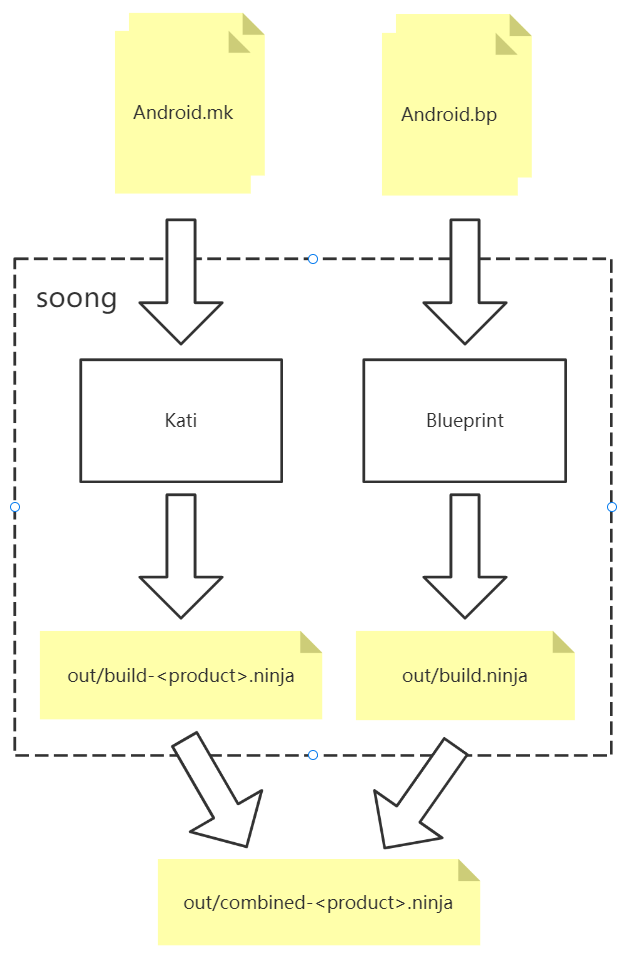
\includegraphics[width=.4\textwidth]{figures/soong-arch.png}
    \caption{soong 构建系统工作示意图}
    \label{fig:soong-architecture}
\end{figure}

对于当前版本的 soong 构建系统而言,其在构建方面主要由 Blueprint 与 Kati 两个转换工具构成——前者负责使用 soong\_ui 生成的 Android.bp.list 文件收集各模块下的 Android.bp 文件并生成 build.ninja,后者负责收集各模块下仍未调整至 Android.bp 文件的 Android.mk 文件并生成 build-<product>.ninja。这两份 ninja 文件是 AOSP 构建对应目标的清单文件,其中详细叙述了该目标可能需要的所有构建过程。

此后,soong 会将二者使用 subninja 语法链接到名为 combined-<product>.ninja 文件中,并将该文件输入至 Ninja,作为 Ninja 开展 AOSP 构建过程的输入之一。在 soong 运行的最后阶段,soong 会创建 Ninja 进程,使用先前生成的 combined-<product>.ninja 文件开始 AOSP 的构建。soong 的整体架构如图 \ref{fig:soong-architecture} 所示。

\subsection{对 AOSP 展开分析的重要性}

在 Google 公司的主导下,AOSP 的维护行为十分频繁,对主要核心仓库的代码变动较大。根据 Google 的 Android Git repositories 中记载,仅 frameworks/base 仓库在 android-12.0.0\_r1 与 android-11.0.0\_r35 两个版本之间就有 151234 个提交记录,其中含有 21611 个非合并提交。其中,存在部分提交涉及数十个文件的核心代码变更。

当前活跃于市场的大多数 Android 手机的核心系统都是基于 AOSP 进一步开发。然而,在 Google 公司发布 AOSP 新版本时,各大公司均需要合入 Google AOSP 的软件变更,这为基于 AOSP 的移动系统研发部门带来了相当大的挑战。

\subsection{分析 AOSP 过程中遭遇的困难}

AOSP 作为 Android 系统的核心组成部分,是一个复杂的整体概念。对其直接展开分析是极其困难的。在对 AOSP 的整体架构进行学习之后,我主要总结出以下三点困难。这三点困难使得对 AOSP 的分析相对于其他软件项目(如 Java Web 项目、Android 应用等)更为复杂。

\begin{itemize}
    \item 独特的构建系统:Android Marshmallow 后,Google 公司选用 soong 作为 AOSP 的顶层构建系统来代替 GNU Make,并使用 ninja 作为底层构建系统加速构建过程。非泛用的构建系统为基于 AOSP 的变更分析带来了设计上的特殊性。
    \item 丰富的编程语言:AOSP 中掺杂了多种通用编程语言,包括但不限于 C,C++,Java,Kotlin,Go,Python 等。编程语言的不统一为基于源代码的分析带来了相当的复杂性。以编程语言多样性相呼应的,是项目结构的多样性。AOSP 由成千上万个不同的项目共同构成,不同的语言所使用的项目结构规范也都不相同,这使得目前许多软件分析工具无法胜任全部工作,必须针对具体情况展开具体分析。
    \item 庞大的系统架构:以 platform/frameworks 为例,其由 67 个仓库组成,共有 5804 个模块,而 AOSP 共拥有数千个代码仓库。与代码仓库数目众多相匹配的,是 AOSP 高度活跃的社区。在 Google 的带领下,大版本间代码变动大成为了 AOSP 的特性之一。
\end{itemize}
